%% Just added files from R Project to Overleaf.

\documentclass[a4paper]{report}
\usepackage[utf8]{inputenc}
\usepackage[T1]{fontenc}
\usepackage{RJournal}
\usepackage{amsmath,amssymb,array}
\usepackage{booktabs}


%% load any required packages here

\usepackage{algorithm}
\usepackage{xcolor}
\usepackage{tabularray}
\usepackage{colortbl}
\usepackage{graphicx}
\usepackage{algpseudocode}

%%%%%%%%%%%%%%%%%%%%%%%%%%%%%%%%%%%%
\usepackage[normalem]{ulem}
\usepackage{xcolor}

% Basic latexdiff commands
\providecommand{\DIFadd}[1]{{\color{blue}#1}}
\providecommand{\DIFdel}[1]{{\color{red}\sout{#1}}}
\providecommand{\DIFaddbegin}{}
\providecommand{\DIFaddend}{}
\providecommand{\DIFdelbegin}{}
\providecommand{\DIFdelend}{}

% Float-safe latexdiff commands
\providecommand{\DIFaddFL}[1]{{\color{blue}#1}}
\providecommand{\DIFdelFL}[1]{{\color{red}\sout{#1}}}
\providecommand{\DIFaddbeginFL}{}
\providecommand{\DIFaddendFL}{}
\providecommand{\DIFdelbeginFL}{}
\providecommand{\DIFdelendFL}{}

%%%%%%%%%%%%%%%%%%%%%%%%%%%%%%%%%%%%%

\usepackage{booktabs}
\usepackage{multirow}

\usepackage{titlesec}
\renewcommand\thesection{\arabic{section}}



% special symbols and abbreviations
% Sets or statistical values
\def\sI{{\mathcal I}}                            % Current Index set
\def\mJ{{\mathcal J}}                            % Select Index set
\def\sL{{\mathcal L}}                            % Likelihood
\def\sl{{\ell}}                                  % Log-likelihood
\def\sN{{\mathcal N}}
\def\sS{{\mathcal S}}
\def\sP{{\mathcal P}}
\def\sQ{{\mathcal Q}}
\def\sB{{\mathcal B}}
\def\sD{{\mathcal D}}
\def\sT{{\mathcal T}}
\def\sE{{\mathcal E}}
\def\sF{{\mathcal F}}
\def\sC{{\mathcal C}}
\def\sO{{\mathcal O}}
\def\sH{{\mathcal H}}
\def\sR{{\mathcal R}}
\def\mJ{{\mathcal J}}
\def\sCP{{\mathcal CP}}
\def\sX{{\mathcal X}}
\def\sA{{\mathcal A}}
\def\sZ{{\mathcal Z}}
\def\sM{{\mathcal M}}
\def\sK{{\mathcal K}}
\def\sG{{\mathcal G}}
\def\sY{{\mathcal Y}}
\def\sU{{\mathcal U}}


\def\sIG{{\mathcal IG}}


\def\cD{{\sf D}}
\def\cH{{\sf H}}
\def\cI{{\sf I}}

% Vectors
\def\vectorfontone{\bf}
\def\vectorfonttwo{\boldsymbol}
\def\va{{\vectorfontone a}}                      %
\def\vb{{\vectorfontone b}}                      %
\def\vc{{\vectorfontone c}}                      %
\def\vd{{\vectorfontone d}}                      %
\def\ve{{\vectorfontone e}}                      %
\def\vf{{\vectorfontone f}}                      %
\def\vg{{\vectorfontone g}}                      %
\def\vh{{\vectorfontone h}}                      %
\def\vi{{\vectorfontone i}}                      %
\def\vj{{\vectorfontone j}}                      %
\def\vk{{\vectorfontone k}}                      %
\def\vl{{\vectorfontone l}}                      %
\def\vm{{\vectorfontone m}}                      % number of basis functions
\def\vn{{\vectorfontone n}}                      % number of training samples
\def\vo{{\vectorfontone o}}                      %
\def\vp{{\vectorfontone p}}                      % number of unpenalized coefficients
\def\vq{{\vectorfontone q}}                      % number of penalized coefficients
\def\vr{{\vectorfontone r}}                      %
\def\vs{{\vectorfontone s}}                      %
\def\vt{{\vectorfontone t}}                      %
\def\vu{{\vectorfontone u}}                      % Penalized coefficients
\def\vv{{\vectorfontone v}}                      %
\def\vw{{\vectorfontone w}}                      %
\def\vx{{\vectorfontone x}}                      % Covariates/Predictors
\def\vy{{\vectorfontone y}}                      % Targets/Labels
\def\vz{{\vectorfontone z}}                      %

\def\vone{{\vectorfontone 1}}
\def\vzero{{\vectorfontone 0}}

\def\valpha{{\vectorfonttwo \alpha}}             %
\def\vbeta{{\vectorfonttwo \beta}}               % Unpenalized coefficients
\def\vgamma{{\vectorfonttwo \gamma}}             %
\def\vdelta{{\vectorfonttwo \delta}}             %
\def\vepsilon{{\vectorfonttwo \epsilon}}         %
\def\vvarepsilon{{\vectorfonttwo \varepsilon}}   % Vector of errors
\def\vzeta{{\vectorfonttwo \zeta}}               %
\def\veta{{\vectorfonttwo \eta}}                 % Vector of natural parameters
\def\vtheta{{\vectorfonttwo \theta}}             % Vector of combined coefficients
\def\vvartheta{{\vectorfonttwo \vartheta}}       %
\def\viota{{\vectorfonttwo \iota}}               %
\def\vkappa{{\vectorfonttwo \kappa}}             %
\def\vlambda{{\vectorfonttwo \lambda}}           % Vector of smoothing parameters
\def\vmu{{\vectorfonttwo \mu}}                   % Vector of means
\def\vnu{{\vectorfonttwo \nu}}                   %
\def\vxi{{\vectorfonttwo \xi}}                   %
\def\vpi{{\vectorfonttwo \pi}}                   %
\def\vvarpi{{\vectorfonttwo \varpi}}             %
\def\vrho{{\vectorfonttwo \rho}}                 %
\def\vvarrho{{\vectorfonttwo \varrho}}           %
\def\vsigma{{\vectorfonttwo \sigma}}             %
\def\vvarsigma{{\vectorfonttwo \varsigma}}       %
\def\vtau{{\vectorfonttwo \tau}}                 %
\def\vupsilon{{\vectorfonttwo \upsilon}}         %
\def\vphi{{\vectorfonttwo \phi}}                 %
\def\vvarphi{{\vectorfonttwo \varphi}}           %
\def\vchi{{\vectorfonttwo \chi}}                 %
\def\vpsi{{\vectorfonttwo \psi}}                 %
\def\vomega{{\vectorfonttwo \omega}}             %


% Matrices
%\def\matrixfontone{\sf}
%\def\matrixfonttwo{\sf}
\def\matrixfontone{\bf}
\def\matrixfonttwo{\boldsymbol}
\def\mA{{\matrixfontone A}}                      %
\def\mB{{\matrixfontone B}}                      %
\def\mC{{\matrixfontone C}}                      % Combined Design Matrix
\def\mD{{\matrixfontone D}}                      % Penalty Matrix for \vu_J
\def\mE{{\matrixfontone E}}                      %
\def\mF{{\matrixfontone F}}                      %
\def\mG{{\matrixfontone G}}                      % Penalty Matrix for \vu
\def\mH{{\matrixfontone H}}                      %
\def\mI{{\matrixfontone I}}                      % Identity Matrix
\def\mJ{{\matrixfontone J}}                      %
\def\mK{{\matrixfontone K}}                      %
\def\mL{{\matrixfontone L}}                      % Lower bound
\def\mM{{\matrixfontone M}}                      %
\def\mN{{\matrixfontone N}}                      %
\def\mO{{\matrixfontone O}}                      %
\def\mP{{\matrixfontone P}}                      %
\def\mQ{{\matrixfontone Q}}                      %
\def\mR{{\matrixfontone R}}                      %
\def\mS{{\matrixfontone S}}                      %
\def\mT{{\matrixfontone T}}                      %
\def\mU{{\matrixfontone U}}                      % Upper bound
\def\mV{{\matrixfontone V}}                      %
\def\mW{{\matrixfontone W}}                      % Variance Matrix i.e. diag(b'')
\def\mX{{\matrixfontone X}}                      % Unpenalized Design Matrix/Nullspace Matrix
\def\mY{{\matrixfontone Y}}                      %
\def\mZ{{\matrixfontone Z}}                      % Penalized Design Matrix/Kernel Space Matrix

\def\mGamma{{\matrixfonttwo \Gamma}}             %
\def\mDelta{{\matrixfonttwo \Delta}}             %
\def\mTheta{{\matrixfonttwo \Theta}}             %
\def\mLambda{{\matrixfonttwo \lambda^2}}           % Penalty Matrix for \vnu
\def\mXi{{\matrixfonttwo \Xi}}                   %
\def\mPi{{\matrixfonttwo \Pi}}                   %
\def\mSigma{{\matrixfonttwo \Sigma}}             %
\def\mUpsilon{{\matrixfonttwo \Upsilon}}         %
\def\mPhi{{\matrixfonttwo \Phi}}                 %
\def\mOmega{{\matrixfonttwo \Omega}}             %
\def\mPsi{{\matrixfonttwo \Psi}}                 %

\def\mone{{\matrixfontone 1}}
\def\mzero{{\matrixfontone 0}}

% Fields or Statistical
\def\bE{{\mathbb E}}                             % Expectation
\def\bC{{\mathbb C}}                             % Expectation
\def\bS{{\mathbb S}}                             % Expectation
\def\bP{{\mathbb P}}                             % Probability
\def\bR{{\mathbb R}}                             % Reals
\def\bI{{\mathbb I}}                             % Reals
\def\bV{{\mathbb V}}                             % Reals
\def\bN{{\mathbb N}}
\def\bK{{\mathbb K}}
\def\bM{{\mathbb M}}
 

\def\d{\partial}
\def\ds{\displaystyle}


\begin{document}

%% do not edit, for illustration only
\sectionhead{Contributed research article}
\volume{18}
\volnumber{4}
\year{2026}
\month{December}
\setcounter{page}{1}

%% replace RJtemplate with your article
\begin{article}
  % !TeX root = RJwrapper.tex
\title{The Lasso Distribution: Properties, Sampling Methods, and Applications in Bayesian Lasso Regression}
\author{by Mohammad Javad Davoudabadi, Jonathon Tidswell, Samuel Muller,  Garth Tarr and John T. Ormerod}

\maketitle



\abstract{
In this paper, we introduce a new probability distribution, the Lasso distribution. We derive several fundamental properties of the distribution, including closed-form expressions for its moments and moment-generating function. Additionally, we present an efficient and numerically stable algorithm for generating random samples from the distribution, facilitating its use in both theoretical and applied settings. We also establish that the Lasso distribution belongs to the exponential family.  A direct application of the Lasso distribution arises in the context of an existing Gibbs sampler, where the full conditional distribution of each regression coefficient follows this distribution. This leads to a more computationally efficient and theoretically grounded sampling scheme. To facilitate the adoption of our methodology, we provide an R package, BayesianLasso, available on CRAN, implementing the proposed methods. Our findings offer new insights into the probabilistic structure underlying the Lasso penalty and provide practical improvements in Bayesian inference for high-dimensional regression problems.   
}

%Introductory section which may include references in parentheses
%\citep{R}, or cite a reference such as \citet{R} in the text. 
\section{Introduction}
The Lasso (Least Absolute Shrinkage and Selection Operator) regression method, introduced by \citet{tibshirani1996regression}, has become a cornerstone in high-dimensional statistical modeling due to its ability to perform variable selection and regularization simultaneously. The Bayesian formulation of the Lasso has been extensively studied, often relying on a Laplace prior for the regression coefficients, which can be expressed as a scale mixture of a Gaussian distribution \citep{park2008bayesian}. However, despite its widespread use, existing formulations often face computational challenges, particularly in efficiently sampling from full conditional distributions in a Gibbs sampling framework \citep{hans2009bayesian}.

In this paper, we propose a new probability distribution, referred to as the Lasso distribution, which arises naturally in the Bayesian formulation of Lasso regression. We fully develop this distribution and derive several of its key properties, including moments, a moment-generating function, and an efficient, numerically stable method for sampling from it. 
Key to these derivations is the accurate and numerically stable evaluation of the Mills ratio that arises in several of these functions \citep{Mills1926}. 
Further, we establish that the Lasso distribution belongs to the class of exponential family distributions, making it a theoretically attractive choice for modeling and inference. 
It is important to note that our formulation of the Lasso distribution differs from the one implemented in the \CRANpkg{LaplacesDemon} package \citep{LaplacesDemon}, which instead corresponds to the scale mixture of normals prior used in \citet{park2008bayesian}.

As an application of the Lasso distribution, we note that it arises naturally as part of a Gibbs sampling scheme, where each coefficient is sampled individually \citep[see][]{hans2009bayesian}. By leveraging the Lasso distribution as the full conditional distribution for the regression coefficients, we achieve a computationally efficient 
%and theoretically grounded 
sampling scheme. To facilitate reproducibility and practical implementation, we provide an R package that implements our proposed methods.


The remainder of the paper is structured as follows. Section \ref{Sec:Bayes_Lasso} outlines our Bayesian hierarchical model, which motivates the Lasso distribution. In Section \ref{Sec:LassoDistribution}, we introduce the Lasso distribution. In Section \ref{sec:lasso_samples}, we describe how to sample efficiently in a numerically stable manner from the Lasso distribution. Section \ref{Sec:UsingBayesPackage} describes how to use the package \CRANpkg{BayesianLasso}. An application of the Lasso distribution via Gibbs sampling is given in Section \ref{Sec:Gibbs}. We present a performance comparison on benchmark datasets in  Section \ref{Sec:Results} and conclude with a brief discussion in Section \ref{Sec:discussion}. 




%%%%%%%% The Bayesian Lasso %%%%%%%%%%%%%%%%%%%%%%%%%%%%%%%%%%%%%%%%%%%%%%%%%%%%%%%%


\section{The Bayesian Lasso}
\label{Sec:Bayes_Lasso}

We consider the standard linear regression model $\vy|\vbeta,\sigma^2 \sim \mathcal{N}(\mX\vbeta, \sigma^2 \mI_n)$ for the observed dataset $\sD = \{\vy, \mX \}$, where $\vy$ is an $n$-dimensional vector of centered responses, $\mX$ is an $n \times p$ matrix of standardized predictors, $\vbeta$ is a $p$-dimensional vector of regression coefficients, and $\sigma^2$ denotes the residual variance parameter. In practice, it is often desirable to perform variable selection alongside parameter estimation, particularly when many covariates may be irrelevant. To this end, \citet{tibshirani1996regression} proposes  Lasso penalized regression, which introduces an $\ell_1$ penalty to encourage sparsity in the estimated coefficients. The regularization strength is governed by a non-negative tuning parameter $\lambda$. The  prior structure 

\begin{equation}\label{eq:aux_representation}
\beta_j| \sigma^2, \tau_j 
    \sim N( 0, \sigma^2 \tau_j),
\quad \mbox{and} \quad
\tau_j 
    \stackrel{\text{iid}}{\sim} \text{Gamma}(1,\lambda^2/2), 
\quad 1\leq j \leq p.
\end{equation}

\noindent 
mimics this penalty when the auxiliary parameter $\tau_j$ is marginalized out \citep{park2008bayesian}.
This hierarchical representation allows for full posterior inference while promoting sparsity through the prior structure. Here, we adopt independent conjugate priors for $\sigma^2$ and $\lambda^2$: $
\sigma^2 \sim \text{IG}(\widetilde{a}, \widetilde{b})$
and $\lambda^2 \sim \mbox{Gamma}(\widetilde{u},\widetilde{v})$
where $\widetilde{a}>0$, $\widetilde{b}>0$, $\widetilde{u}>0$, and $\widetilde{v}>0$ are fixed prior hyperparameters.

We propose a modification to the hierarchical prior model in \eqref{eq:aux_representation} that introduces a different auxiliary-variable representation. Specifically, instead of the local scale parameter 
$\tau_j$ used in \eqref{eq:aux_representation}, we introduce the variable $\eta_j$ and express the prior for $\beta_j$ through the alternative hierarchical formulation
\begin{equation}\label{equ3}
\beta_j | \sigma^2, \eta_j 
    \sim N\left( 0, \frac{\sigma^2}{\eta_j\lambda^2} \right),
\quad \text{and} \quad
\eta_j \stackrel{\text{iid}}{\sim} \text{IG}(1, 1/2), \quad 1 \leq j \leq p.
\end{equation}

This representation is not identical to \eqref{eq:aux_representation} but is constructed so that the resulting full conditional distribution of $\beta_j$ admits the kernel form given in \eqref{LassoProp}, which facilitates the sampling strategy used in our Gibbs sampler.

\citet{hans2009bayesian} takes a different approach. Instead of using the auxiliary variable representations in \eqref{eq:aux_representation} and \eqref{equ3}, the standard Gibbs sampler of \citet{hans2009bayesian} samples from the full conditional distributions of the parameters individually, employing a weighted combination of two truncated normal distributions. It can be shown that the full conditional distribution for each $\beta_j$ is proportional to 
\begin{align}\label{LassoProp}
p(\beta_j|\sD,\vbeta_{-j},\sigma^2,\lambda^2) \propto 
\exp\left(-\tfrac{1}{2}a\beta_j^2 + b\beta_j - c |\beta_j|\right)
\end{align}
where $a$, $b$, and $c$ 
are constants that
depend on $\sD$, $\vbeta_{-j}$, $\sigma^2$, and $\lambda^2$. 
This kernel corresponds to the weighted combination of two truncated normal distributions utilized by \citet{hans2009bayesian}. Further details can be found in the Supplementary Material.


Although this conditional kernel can be expressed as a weighted mixture of truncated normal distributions and sampled within a Gibbs sampler \citep{hans2009bayesian}, it has not previously been formalized as a standalone distribution with explicitly derived analytical properties. In particular, \citet{hans2009bayesian} utilized the truncated normal mixture representation for computational purposes but did not formally study the kernel as a distinct probability distribution, derive its properties in closed form, or develop numerically stable normalization formulas. To address this challenge, we develop a new distribution, which we term the {\em Lasso distribution}, arising naturally in the context of the Lasso regression model. We establish its analytical properties together with stable computational methods and an accompanying open-source R package implementation. In the next section, we formally define the Lasso distribution and derive several of its key properties, including its probability density function (PDF), cumulative distribution function (CDF), moment generating function (MGF), and moments.



%%%%%%%% The Lasso Distribution %%%%%%%%%%%%%%%%%%%%%%%%%%%%%%%%%%%%%%%%%%%%%%%%%%%%%%%%%%%%%%%%%%%%%%%%%%%%%%%%%%%%

\section{The Lasso distribution}\label{Sec:LassoDistribution}

We derive several properties of the Lasso distribution, including the probability density function (PDF), cumulative density function (CDF), moment generating function (MGF), and moments. For detailed derivations, please refer to Section B of the Supplementary Materials.

% % In this study, we introduce a novel distribution specifically tailored for the Gibbs sampler as the full conditional distribution of the regression coefficients within the framework of the Lasso regression. Our goal is to leverage this distribution to facilitate shrinkage and improve the performance of the Gibbs sampler in estimating the regression coefficients.

% The introduced distribution is designed to incorporate shrinkage properties, allowing for more effective regularization and variable selection. By utilizing this distribution within the Gibbs sampler, we can draw samples from it to update the regression coefficients iteratively. This approach ensures that the resulting estimates exhibit desirable shrinkage properties, promoting sparsity and reducing the impact of irrelevant variables.

A random variable $X$ that maps from a probability space to the real line $\mathbb{R}$ has a Lasso distribution with parameters $a$, $b$, and $c$, denoted $X \sim \text{Lasso}(a,b,c)$, if its PDF is 
\begin{align*}
   p(X,a,b,c) = Z^{-1}\exp\left(-\tfrac{1}{2}aX^2+bX-c|X|\right),
\end{align*}
where $a \geq 0$, $b \in \mathbb{R}$, $c \geq 0$ (with $a$ and $c$ not both 0), and normalizing constant  $Z$   given by
$$Z(a,b,c) = \int_{-\infty}^\infty \exp\left( -\tfrac{1}{2}aX^2 + bX - c|X| \right) dx = \sigma \left[ \frac{\Phi(\mu_1/\sigma)}{\phi(\mu_1/\sigma)}
+ \frac{\Phi(-\mu_2/\sigma)}{\phi(-\mu_2/\sigma)}  \right],$$
with $\mu_1 = (b-c)/a$, $\mu_2 = (b + c)/a$, and $\sigma^{2} = 1/a$. Here, $\Phi(\cdot)$ and $\phi(\cdot)$ denote the CDF and PDF of the standard normal distribution, respectively. The parameter $a$ controls the quadratic curvature of the density and governs its overall concentration. The parameter $b$ introduces a linear tilt, inducing asymmetry and shifting mass toward positive or negative values. The parameter $c$ controls the strength of the absolute value term, increasing concentration near zero and producing the characteristic cusp of the Lasso distribution.
Evaluating $Z$ can be numerically challenging due to potential overflow, underflow, or divide-by-zero problems. To address this, our R package \CRANpkg{BayesianLasso} implements a numerically stable and efficient method for computing $Z$, automatically managing these numerical difficulties \citep{BayesianLassoPkg}.



%$Z$ is a function of the Mill's ratio, $m(x) = (1 - \Phi(x))/\phi(x)$. 

%We will address these problems in Section \ref{sec:lasso_samples} of the Supplementary materials.


The Lasso distribution can be written as a mixture of two truncated normal distributions.
As we shall see, for different extreme values of $a$, $b$ and $c$, the Lasso distribution can behave like a normal distribution, a Laplace distribution, an asymmetric Laplace distribution, a positively truncated normal distribution, or a negatively truncated normal distribution. 
By characterizing the limiting behavior under extreme parameter values, the R package \CRANpkg{BayesianLasso} leverages appropriate approximations to known distributions ensuring robust and efficient computation even in numerically challenging settings.
Figure \ref{fig:density_Lassos} shows the density of the univariate Lasso distribution for different parameter values. 

\begin{figure}[ht]
    \centering
    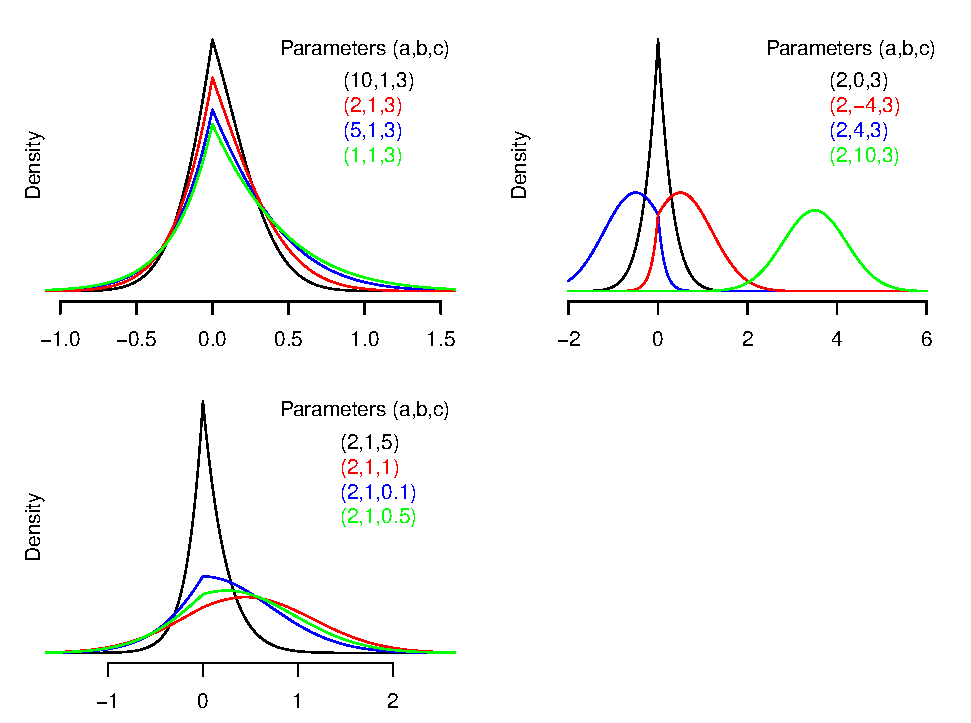
\includegraphics[width=15cm, height=12.2cm]{figures/bayesianlasso.pdf}
    \vspace*{-0.5cm}
    \caption{The Lasso density function is depicted for different parameter values. In the top left panel, parameter $a$ is varied while the other parameters are fixed. In the top right and bottom left panels, parameters $b$ and $c$ are varied, respectively, while the other parameters are fixed.}
    \label{fig:density_Lassos}
\end{figure}






% Here, the log-partition function is
% \begin{align*}
%     A(\theta ) = \log(Z) &= \log(\int h(x)\exp(\nu(\theta) T(x))dx)\\&
%     =\log(\int \exp(-\frac{1}{2}ax^2+bx-c|x|)dx).
% \end{align*}

The MGF of the Lasso distribution is $M(t) = Z(a,b+t,c)/Z(a,b,c)$ and the calculation of the moments of the Lasso distribution via the MGF is algebraically cumbersome. See Section B of the Supplementary Materials for the derivation of the MGF. However, by expressing the Lasso distribution as a mixture of two truncated normal distributions, the moments can be calculated as $
    \mathbb{E}(X^r) = (1 - w) \cdot \mathbb{E}(A^r) + w  \cdot \mathbb{E}(B^r),
$ where the mixing proportion is given by
$$
w =  \left[ 1
+ \frac{\Phi(\mu_1/\sigma)}{\phi(\mu_1/\sigma)}\frac{\phi(-\mu_2/\sigma)}{\Phi(-\mu_2/\sigma)}
\right]^{-1}, 
$$
where $A\sim TN_+(\mu_1,\sigma^{2})$ and $B\sim TN_-(\mu_2,\sigma^{2})$ are the positively truncated and negatively truncated normal distributions, respectively. 

The CDF of the Lasso distribution is given by
$$
\displaystyle 
P(x) = \mathcal{P}(X < x) 
     = \left\{ \begin{array}{ll}
\displaystyle 
w\frac{\Phi\left( 
\frac{x - \mu_2}{\sigma}\right)}{\Phi(-\mu_2/\sigma)} 
    & \mbox{if $x\le 0$ and}
\\ [2ex]
\displaystyle  1 - (1 - w)\frac{\Phi(\frac{\mu_1 - x}{\sigma})}{\Phi(\mu_1/\sigma)}
    & \mbox{if $x> 0$}.
\end{array} 
\right.
$$
 
The inverse CDF of the Lasso distribution is given by
\begin{align}\label{equ:inv_CDF}
    P^{-1}(u) = \left\{
\begin{array}{ll}
\mu_2 + \sigma\Phi^{-1}[\Phi(-\mu_2/\sigma) u/w] 
    & \mbox{if $u\le w$ and} 
\\ [2ex]
\mu_1 - \sigma\Phi^{-1}[\Phi(\mu_1/\sigma) (1 - u)/(1-w) ]
    & \mbox{if $u> w$}.
\end{array} 
\right.
\end{align}
Finally, the mode of the Lasso distribution is equal to $\mbox{max}(|b| - c,0)\cdot\mbox{sign}(b)/a$, where $\mbox{sign}(\cdot)$ is the sign function. 

The R package \CRANpkg{BayesianLasso} enables efficient and numerically stable sampling from the Lasso distribution by evaluating the inverse CDF using uniform random draws. To ensure robustness, particularly in the tails, the implementation incorporates safeguards against numerical issues such as overflow and underflow. A key component of this approach is the numerically stable evaluation of the Mills ratio, defined as $m(x) = \Phi(-x)/\phi(-x)$, which is used in computing the normalizing constant. Specifically, the package computes 
$$
v_{1}=\frac{c-\left|b\right|}{\sqrt{a}} 
\qquad 
\mbox{and} \qquad  
v_{2}=\frac{c+\left|b\right|}{\sqrt{a}},
$$ 
and evaluates the normalizing constant as
$Z = \left[m\left(v_{1}\right)+m\left(v_{2}\right)\right]/\sqrt{a}$. This combination of numerical stability and computational efficiency underpins the practical value of the package and is a key reason for its robustness in high-dimensional Bayesian inference.




%%%% Sampling from the Lasso distribution  %%%%%%%%%%%%%%%%%%%%%%%%%%%%%%%%%%%%%%%%%%%%%%%%%%%%%%%%%%%%%%%%%%%%%%%%%%%%%%%%%%%%



\subsection{Sampling from the Lasso distribution}
\label{sec:lasso_samples}

Key quantities required for various expressions in the previous section include the computation of $Z$ and $w$. Additionally, special care must be taken when calculating the inverse CDF to prevent both overflow and underflow. To address these concerns, we define $
v_{1}=\left(c-\left|b\right|\right)/\sqrt{a}$ and $ 
v_{2}=\left(c+\left|b\right|\right)/\sqrt{a}$. The normalizing constant 
$Z$ can then be expressed as
$Z = \left[m\left(v_{1}\right)+m\left(v_{2}\right)\right]/\sqrt{a}$.
For negative inputs, i.e., $x<0$, the Mills ratio is 
$m\left(x\right)=\phi\left(x\right)^{-1}-m\left(-x\right)$. Since $v_{2}\ge 0$ and $v_{1}\ge 0$ when $\left|b\right|\le c$, we can partition the definition of $Z$ into two cases
\begin{align*}
Z & =\begin{cases}
\frac{1}{\sqrt{a}}\left[m\left(v_{1}\right)+m\left(v_{2}\right)\right] & \left|b\right|\le c \quad \mbox{and}\\
\frac{1}{\sqrt{a}}\left[\left(\phi\left(v_{1}\right)^{-1}-m\left(-v_{1}\right)\right)+m\left(v_{2}\right)\right] & \left|b\right|>c;
\end{cases}
\end{align*}
where both alternatives have the requirement for two Mills ratio
calculations for positive parameters; this is a potential use case
for a SIMD, which is short for single instruction/multiple data, vectorized implementation of the positive side of the Mills ratio. 

The second component of $Z$ (for $\left|b\right|>c$) has an obvious
potential overflow when $\left|v_{1}\right|$ is large.  In such cases, it may be necessary to transition to logarithmic space to represent $\phi\left(v_{1}\right)$
to avoid underflow/overflow.
However, unnecessary logarithmic computations should be avoided, as they are computationally expensive and can reduce numerical precision when not required. \citet{marsaglia2004evaluating} notes that the precision of evaluating the standard normal density function $\phi\left(x\right)$ and its tail probability deteriorates as 
$x$ increases, due to the limitations of computing $\exp(-x^2/2)$ in double-precision arithmetic. While the paper primarily examines values up to $x \approx 16$, it is also known that $\phi\left(x\right)$ effectively loses all precision for $x\geq 37$ , where the exponential term underflows to zero and the reciprocal overflows. Now, consider the case where $v_{1}<-37$, making overflow a concern. 
By definition, we have $37<-v_{1}<v_{2}$, which implies $m\left(37\right)>m\left(-v_{1}\right)>m\left(v_{2}\right)>0$. Since $m\left(37\right)\approx0.027$, it follows that  $-0.027<m\left(v_{2}\right)-m\left(-v_{1}\right)<0$. Within the limits of double precision, this difference becomes negligible due to rounding errors for $v_{1}\approx-9$, and certainly for $v_{1}<-37$, where $\phi\left(-37\right)<6\times10^{-300}$. Consequently, $Z$ can be approximated as
\begin{align*}
Z & \approx\frac{1}{\sqrt{a}}\left[\phi\left(v_{1}\right)^{-1}\right].
\end{align*}
 Thus, we can safely use the approximation $m\left(v_{1}\right)\approx\phi\left(v_{1}\right)^{-1}$ in such cases.




For a fast and accurate approximation of Mills ratio for positive arguments, we employ a degree $\left(8,9\right)$ rational polynomial optimized using the Remez algorithm \citep{reemtsen1990modifications} over the interval $\left[0,600\right]$, achieving an accuracy of up to 12 significant figures. The leading coefficients of both the numerator and denominator are positive, ensuring that the approximation asymptotically converges to a small fraction. This stability allows the relative error to remain consistent, preserving 11  significant figures up to approximately $x\approx2000$. Beyond this point, the precision gradually improves, as Mills ratio satisfies $m(x) \sim 1/x$ for large $x$.

Let 
$$
\begin{array}{c}
p_0 = 46697.7602201933, \qquad  p_1 = 69339.6909002865, \qquad p_2 =50590.6980372328, \\
p_3 = 23184.62760379742, \qquad p_4 = 7236.31450136984, \qquad p_5 = 1572.136841909630, \\ 
p_6 = 232.9967987466022, \qquad p_7 = 21.74833514806325, \qquad \mbox{and} \quad p_8 = 1.000000000000095.
\end{array}
$$
and let
$$
\begin{array}{c}
q_0 = 37259.42190376593, \qquad q_1 = 85053.78630172011, \qquad q_2 = 89598.92885811838, \\
q_3 = 57370.93777717682, \qquad q_4 = 24713.27114352290, \qquad q_5 = 7467.311205544661, \\ 
q_6 = 1593.885178714749, \qquad q_7 = 233.9967987305447, \qquad q_8 = 21.74833514813385, \\
\end{array}
$$
and $q_{9} = 1$. Let
$$
\displaystyle \widetilde{m}  = \frac{
    p_0 + x(p_1 + x(p_2 + x( p_3 + x(p_4 + x(p_5 + x(p_6 + x(p_7 + xp_8)))))))
}{
    q_0 + x(q_1 + x(q_2 + x(q_3 + x(q_4 + x(q_5 + x(q_6 + x(q_7 + x(q_8 + x))))))))
}.
$$
Our approximation of $m(x)$ for $x>0$ is then
$$
m(x) = \left\{\begin{array}{ll}
\widetilde{m}    & \mbox{$x < 1.75 \times 10^{34}$} \\
1/x  & \mbox{otherwise.}
\end{array}\right.
$$


Next, we define 
$$
w_{1}=\frac{1}{1+m\left(v_{1}\right)m\left(v_{2}\right)^{-1}}
\qquad 
\mbox{and}
\qquad 
w_{2}=\frac{1}{1+m\left(v_{1}\right)^{-1}m\left(v_{2}\right)}.
$$
As $v_{1}\rightarrow-\infty$, it follows that $m\left(v_{1}\right)\rightarrow\infty$, leading to $w_{1}\rightarrow0$ and $w_{2}\rightarrow1$.
However, due to the dynamic range limitations of floating-point representation, $w_{1}$
is representable, whereas  $w_{2}$ rounds to 1 for $v_{1}\lessapprox-5.5$,
resulting in a loss of precision. Since floating-point arithmetic offers much better precision near zero than near one, using $w_{2}$ when $v_{1}\ll0$ can introduce numerical errors. To mitigate this, we define
$$
w=\begin{cases}
w_{1} & \mbox{if } b\le0 \mbox{ and} \\
w_{2} & \mbox{if } b>0,
\end{cases}
\qquad \mbox{and}
\qquad 
1-w =\begin{cases}
w_{2} & \mbox{if } b\le0 \mbox{ and} \\
w_{1} & \mbox{if } b>0.
\end{cases}
$$
Thus, a simple yet numerically stable rule is to work with $w$ when $b\le0$ and with $1-w$
when $b>0$.

The computation of $P^{-1}(u)$ is carried out in four distinct cases, determined by whether $u \leq w$ and whether $b > 0$. First, the arguments of $\Phi^{-1}(\cdot)$ are carefully computed to prevent overflow. In extreme cases, underflow may still occur. When underflow is detected, the arguments of $\Phi^{-1}(\cdot)$ are instead computed on the logarithmic scale, and the asymptotic tail formula of \citet{Martin} is used to evaluate $\Phi^{-1}(\cdot)$ accurately.



%%%%%% Code example of the Lasso distribution %%%%%%%%%%%%%%%%%%%%%%%%%%%%%%%%%%%%%%%%%%%%%%%%%%%%%%%%%%%%%%%%%%%%%%%%%%

\section{Using the BayesianLasso package}\label{Sec:UsingBayesPackage}

To illustrate the functionality of the \CRANpkg{BayesianLasso} package, we provide examples of its key functions, including density evaluation, cumulative distribution, random sampling, and quantile calculations.

\subsection{Probability density function (PDF)}

The function \code{dlasso()} computes the probability density function of the Lasso distribution for given parameters. The following example plots the density of a $\text{Lasso(2,1,3)}$ distribution, shown as a solid black line in Figure \ref{fig:density_comparison}.

\begin{example}
library(BayesianLasso)

# Define parameters
a <- 2
b <- 1
c <- 3
x <- seq(-3, 3, length = 1000)

# Plot the density of Lasso(2,1,3)
plot(x, dlasso(x, a, b, c, logarithm = FALSE), type = 'l', 
     xlab = "x", ylab = "Density", 
     ylim = c(0, 2.25), yaxt = "n", bty = "n")
\end{example}



\subsection{Cumulative distribution function (CDF)}
The function \code{plasso()} calculates the cumulative distribution function of the Lasso distribution. Below, we compute the CDF at $x = -1$ for a $\text{Lasso}(2,1,3)$ distribution:

\begin{example}
CDF_value <- plasso(-1, a, b, c)
print(CDF_value)
[1] 0.00176594
\end{example}

\subsection{Random sampling from the Lasso distribution}
To generate random samples from the Lasso distribution, we use \code{rlasso()}. The following example generates 100,000 samples and compares the empirical density with the theoretical density, as shown in Figure \ref{fig:density_comparison}.

\begin{example}
# Generate random samples
samples <- rlasso(100000, a, b, c)

# Compare empirical and theoretical density
plot(x, dlasso(x, a, b, c, logarithm = FALSE), type = "l", lty = 1,
     xlab = "x", ylab = "Density",
     xlim = c(-2, 2), yaxt = "n", bty = "n")
lines(density(samples), col = "red", type = "l", lty = 2)

legend("topright", legend = c("Theoretical", "Empirical"), col = c("black", "red"),
       lty = c(1, 2), bty = "n")
\end{example}

\begin{figure}[ht]
    \centering
    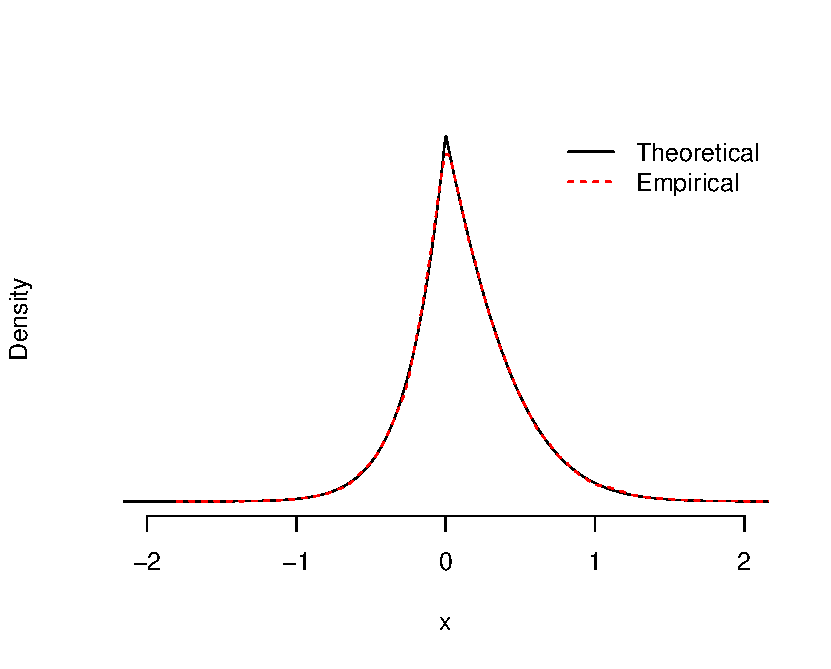
\includegraphics[width=10cm, height=8cm]{figures/sampling_lassoDist.pdf}
    \vspace*{-0.5cm}
    \caption{Theoretical and empirical densities for $\text{Lasso}(2,1,3)$. The theoretical density plot of $\text{Lasso}(2,1,3)$ using \code{dlasso(x, a, b, c, logarithm = FALSE)} is shown as a solid black line, and the empirical density is shown as a dashed line.}
    \label{fig:density_comparison}
\end{figure}



To assess implementation accuracy, we compare empirical moments obtained from Monte Carlo simulation with the theoretical mean, \texttt{elasso(a,b,c)}, and variance, \texttt{vlasso(a,b,c)}, derived in Section~\ref{Sec:LassoDistribution}. For multiple parameter configurations $(a,b,c)$ chosen to represent different scales and degrees of concentration, $10^5$ independent samples were generated using \texttt{rlasso()}. The empirical mean and variance were computed and compared with their analytical counterparts, and the absolute errors between theoretical and empirical moments are reported in Table~\ref{tab:moment_comparison}.

\begin{table}[ht]
\centering
\begin{tabular}{c|ccc|ccc}
\hline
$(a,b,c)$ & 
\multicolumn{3}{c|}{Mean} & 
\multicolumn{3}{c}{Variance} \\
\cline{2-7}
 & Theoretical & Empirical & Error & Theoretical & Empirical & Error \\
\hline
$( 2,\, 1,\, 3)$ & 0.121830 & 0.122919 & 0.001088 &  0.128773 & 0.129729 & 0.000955\\
$(4 ,\, 4,\, 1)$ &  0.773432 & 0.773007 & 0.000425 & 0.228095 & 0.226861 & 0.001233 \\
$(1 ,\, 1,\,1 )$ & 0.503222 & 0.503450 & 0.000227 & 0.558956 & 0.559068 & 0.000111 \\
\hline
\end{tabular}
\caption{Comparison of theoretical and empirical moments for selected $(a,b,c)$ parameter settings.}
\label{tab:moment_comparison}
\end{table}

Table~\ref{tab:moment_comparison} demonstrates close agreement between the theoretical and empirical moments across all tested parameter settings. For $10^5$ independent Monte Carlo draws, the empirical means and variances match their analytical counterparts to three or more decimal places, with absolute errors uniformly below $10^{-3}$. The magnitude of these discrepancies is consistent with expected Monte Carlo error, indicating that the random number generator \texttt{rlasso()} and the analytical moment functions \texttt{elasso()} and \texttt{vlasso()} are correctly implemented and numerically stable.

\subsection{Quantile function}
The inverse-CDF sampler corresponding to Equation \eqref{equ:inv_CDF} is implemented in C++ which is located in \texttt{src/lasso\_distribution.cpp}, and is exposed to users via the exported Rcpp interface \code{qlasso()}. The required evaluations of the normal cumulative distribution function 
and its inverse are performed using the R math library routines 
\texttt{R::pnorm5} and \texttt{R::qnorm5}. These routines compute the 
normal CDF and quantile using piecewise rational approximations with 
separate central and tail expansions, ensuring high 
numerical accuracy and stability even for extreme probability values.





Below, we compute the quantiles for probability values \textbf{$p = \{0.1, 0.3, 0.6\}$}:

\begin{example}
p_values <- c(0.1, 0.3, 0.6)
quantiles <- qlasso(p_values, a, b, c)
print(quantiles)
[1] -0.28183916 -0.04935763  0.16137104
\end{example}





\subsection{Numerical stability and boundary behaviour}
\label{sec:numerical_validation}

\paragraph{Failure cases of naive implementations.}
A direct implementation of the Lasso distribution based on the density
\[
f(x \mid a,b,c) \propto \exp\!\left(-\frac{1}{2}ax^2 + bx - c|x|\right)
\]
can suffer from substantial numerical instability. In particular, naive evaluation of the normalizing constant may overflow when $|b|/c$ is large, due to the exponential terms arising from Gaussian tail probabilities. Similarly, direct subtraction of nearly equal floating-point quantities in cumulative distribution function (CDF) computations may lead to catastrophic cancellation in extreme tail regions. 

In addition, straightforward inversion of the CDF for quantile evaluation can fail without careful bracketing, particularly in highly skewed parameter regimes. These issues are common in naive implementations that rely solely on closed-form expressions without attention to floating-point behaviour.

The implementation in \texttt{BayesianLasso} mitigates these problems by performing normalization and tail probability calculations on the log-scale, separating positive and negative domains explicitly, and using numerically stable bracketing procedures for quantile inversion. These design choices ensure stable behaviour across a wide range of parameter values.

\paragraph{Boundary and near-degenerate regimes.}
We further investigated behaviour in limiting parameter regimes:

\begin{itemize}
\item \textbf{$c \to 0$.} In this limit, the Lasso distribution converges to a Gaussian distribution with mean $b/a$ and variance $1/a$. Numerical experiments demonstrate that the implementation transitions smoothly to this Gaussian case without discontinuity or instability.

\item \textbf{$a \to 0$.} As $a$ approaches zero, the quadratic term vanishes and the distribution approaches a Laplace-type density. Direct evaluation of normalization constants becomes ill-conditioned in this regime; however, the log-scale implementation maintains numerical stability and produces accurate density and distribution evaluations.

\item \textbf{Large $|b|/c$.} When $|b|/c$ is large, the distribution becomes highly skewed and naive exponential evaluations may overflow. The current implementation remains stable under such extreme skewness due to its log-scale normalization and careful handling of Gaussian tail probabilities.
\end{itemize}

These investigations demonstrate that the proposed implementation is robust not only in regular parameter settings but also in boundary and numerically challenging regimes. Such stability is essential for reliable use of the Lasso distribution in Bayesian computation and simulation-based inference.


In the next section, we incorporate the Lasso distribution into a Gibbs sampling algorithm as the full conditional distribution for the coefficients of the Lasso regression model.

%%%%% Application of the Lasso Distribution in Gibbs Sampling  %%%%%%%%%%%%%%%%%%%%%%%%%%%%%%%%%%%%%%%%%%%%%%%%%%%%%%%%%%%%%%%%%%%%%%%%%%%%%%%%%%%%

\section{Application of the Lasso distribution in Gibbs sampling}
\label{Sec:Gibbs}

We modify the Gibbs sampler of \citet{hans2009bayesian} (henceforth Hans) by using the Lasso distribution as the full conditional distribution of the regression coefficients. We also consider a slightly modified version of the Gibbs sampler of \citet{park2008bayesian} (henceforth PC), as the alternative Gibbs sampler, by changing the representation of the auxiliary variable from \eqref{eq:aux_representation} to \eqref{equ3}.


Furthermore, these Gibbs samplers are based on the prior $\lambda^2\sim\mbox{Gamma}(\widetilde{u},\widetilde{v})$ which differs from
\citet{hans2009bayesian}, where the prior is placed on $\lambda$ (which is conjugate) rather than $\lambda^2$ (which is not conjugate in the modified Hans sampler). The primary motivation for this choice is to ensure consistency with the parameterization used in the PC Gibbs sampler, which is formulated in terms of $\lambda^2$. This allows us to place both samplers under the same underlying model specification and enables a direct and fair comparison between their sampling strategies. In addition, modeling $\lambda^2$ aligns naturally with the formulation of the Lasso distribution introduced in this paper, where $\lambda^2$ enters directly into the quadratic form of the conditional density. This parameterization therefore provides a more coherent connection between the model and the proposed sampling approach. However, unlike the conjugate specification for $\lambda$ in \citet{hans2009bayesian}, placing the prior on $\lambda^2$ breaks conjugacy, necessitating the use of a slice sampler \citep{neal2003slice} for its full conditional distribution. 


Theoretically, both specifications induce similar shrinkage behavior, but they differ in computational properties. The conjugate prior leads to simpler Gibbs updates, whereas the non-conjugate specification requires auxiliary sampling steps. In practice, this may affect mixing for $\lambda^2$, leading to poorer mixing in some settings (e.g., the Crime dataset in Table \ref{tab:ngtp_results_lasso}), which we regard as a computational trade-off of the chosen parameterization. All methods are implemented in the same programming language and executed on the same computer, ensuring that the primary distinction lies in the choice of Gibbs samplers used to fit the model.




\subsection{Hans Gibbs sampler}

As stated earlier, the standard Gibbs sampler proposed by \citet{hans2009bayesian} relies on the fact that the full conditional distribution for each $\beta_j$ is given by \eqref{LassoProp}, and \citet{hans2009bayesian} 
notes that $p(\beta_j|\sD,\vbeta_{-j},\sigma^2,\lambda^2)$ can be represented as a mixture of two truncated normal distributions. This is not a well-known distribution to sample. However, we show care needs to be taken to avoid numerical problems using this representation.

To facilitate sampling from the kernel in \eqref{LassoProp}, we utilize the Lasso distribution ($\mbox{Lasso}(a,b,c)$), which we introduced in Section \ref{Sec:LassoDistribution}. We also employ the efficient and numerically stable sampling method developed in Section \ref{sec:lasso_samples} to draw samples from this distribution. Notably, while the Hans sampler is specifically designed for the Lasso distribution, it is difficult to extend to other response types or alternative penalty structures.


Algorithm~\ref{B_Gibbs} presents our modified version of Hans’ Gibbs sampling algorithm, where we model $\lambda^2 \sim \mbox{Gamma}(\widetilde{u},\widetilde{v})$ instead of $\lambda \sim \mbox{Gamma}(\widetilde{u},\widetilde{v})$. Unlike the original method in \citet{hans2009bayesian}, which employs conjugate sampling for $\lambda$ and rejection sampling for $\sigma^2$, our approach collapses the auxiliary variable $\eta_j$ to improve mixing and utilizes slice sampling for both $\sigma^2 \mid \sD, \vbeta, \lambda^2$ and $\lambda^2 \mid \sD, \vbeta, \sigma^2$ \citep{neal2003slice}. Notably, the same slice sampler is applied to both parameters, as their full conditional distributions are inverse transformations of each other. 





\begin{algorithm}[!ht]
\caption{Modified Hans Gibbs sampler}\label{B_Gibbs}
\begin{algorithmic}[1]

\State \textbf{Inputs}: $\vy$, $\mX$, $\widetilde{a}>0$, $\widetilde{b}>0$, $\widetilde{u}>0$, $\widetilde{v}>0$, $\vbeta^{(0)} = \vzero_p$, $\sigma^{2(0)}>0$, $\lambda^{(0)}>0$; 

\For {$i = 1,\ldots,\textit{N}$}

\State $\vbeta^{(i)} \leftarrow \vbeta^{(i-1)}$;





\If{$n>p$} 
    \State $\vdelta \leftarrow  (\mX^T\mX) \vbeta^{(i)}$;
    \For {$j = 1,\ldots,\textit{p}$} 
        \State $\vdelta \leftarrow  \vdelta - \mX_j \beta_j^{(i)}$;
        \State $\ds \beta^{(i)}_j \sim 
            \text{Lasso}\left( 
                \frac{\| \mX_j\|_2^2}{\sigma^{2(i-1)}}, 
                \frac{(\mX^T\vy)_j - \delta_j}{\sigma^{2(i-1)}}, 
                \frac{\lambda^{(i-1)}}{\sigma^{(i-1)}} 
            \right);$
        \State $\vdelta \leftarrow  \vr + \mX_j \beta_j^{(i)}$;
    \EndFor
    \State $\mbox{RSS} \leftarrow  \|\vy\|_2^2 - 2\vy^T\mX\vbeta_j^{(i)} + (\vbeta_j^{(i)})^T\mX^T\mX\vbeta_j^{(i)}$;
\Else 
    \State $\vy \leftarrow \mX\vbeta^{(i)}$;

\For {$j = 1,\ldots,\textit{p}$} 
\State $\vr_j \leftarrow \vy - (\widehat{\vy} - \mX_{j}\beta^{(i-1)}_j);$

\State $\ds \beta^{(i)}_j \sim 
    \text{Lasso}\left( 
        \frac{\| \mX_j\|_2^2}{\sigma^{2(i-1)}}, 
        \frac{\mX_j^T\vr_j}{\sigma^{2(i-1)}}, 
        \frac{\lambda^{(i-1)}}{\sigma^{(i-1)}} 
    \right);$

\State $\widehat{\bf y} \leftarrow \widehat{\bf y} + {\bf X}_{j}(\beta^{(i)}_j - \beta^{(i-1)}_j) $;
\EndFor

    \State $\mbox{RSS} \leftarrow  \|\vy - \widehat{\vy}\|_2^2$;

\EndIf


\State Use slice sampling to sample $\sigma^{2(i)}$ from the density
$$
\ds p(\sigma^2|\sD,\vbeta^{(i)},\lambda^{2(i-1)})      
    \propto \exp\left[
        (\widetilde{a} +\tfrac{n+p}{2} +1)\log(\sigma^{2}) 
        - \left(\widetilde{b} + \tfrac{1}{2}\mbox{RSS}\right)\sigma^{-2} - \tfrac{\lambda^{(i-1)}}{\sigma}\| \vbeta^{(i)} \|_1 \right];
$$

\State Use slice sampling to sample $\lambda^{2(i)}$ from the density
$$
\ds p(\lambda^{2}|\sD,{\boldsymbol\beta}^{(i)},\sigma^{2(i)}) 
    \propto \exp\left[
        \left( \widetilde{u} + \tfrac{p}{2} - 1\right) \log(\lambda^{2}) 
        - \widetilde{v}\lambda^{2(i-1)} 
        - \tfrac{\lambda}{\sigma^{(i)}} \| \vbeta^{(i)} \|_1 \right].
$$

\EndFor
\end{algorithmic}
\end{algorithm}


In Algorithm \ref{B_Gibbs}, the quantity ${\bf r}_j$ is analogous to the partial residuals used in coordinate descent methods for optimizing the Lasso objective function \cite[see, e.g.,][Section 5.4.2]{HasteEtAl2015}. However, rather than computing the mode of $\beta_j|{\mathcal D},{\boldsymbol\beta}_{-j},\sigma^2$ as done in coordinate descent, we draw samples from its distribution.

\citet{hans2009bayesian} does not discuss the computational costs of the Gibbs samplers presented there. In contrast, our Algorithm \ref{B_Gibbs} avoids matrix inversion, and as shown in Algorithm \ref{B_Gibbs}, sampling each variable requires $\mathcal{O}(\min(n,p))$  time, assuming the quantities $\mX^T\mX$ (for $n>p$), $\mbox{diag}(\mX^T\mX)$ and $\mX^T\vy$ are computed outside the main loop. Moreover, Algorithm \ref{B_Gibbs} accommodates both the $n>p$ and $p>n$  settings, running in $\mathcal{O}(N p \min(n,p))$ time where $N$ is the number of samples drawn.


Note that our \CRANpkg{BayesianLasso} package implements the modified Hans sampler via the function
\texttt{Modified\_Hans\_Gibbs()}. In this function, $\mX$ and $\vy$ represent the covariate matrix and the response vector, respectively. The arguments \texttt{a1}, \texttt{b1}, \texttt{u1}, and \texttt{v1} correspond to the hyperparameters of the priors for $\sigma^2$ and $\lambda^2$. The total number of MCMC iterations is specified by \texttt{nsamples}, and the initial values for $\vbeta$, $\sigma^2$ and $\lambda^2$ are set via {\tt beta\_init}, \texttt{sigma2\_init} and \texttt{lambda\_init}, respectively. The argument \texttt{verbose} controls whether the sampling progress is printed during execution. The argument \texttt{thin} controls the thinning interval of the MCMC chain. Only every thin-th draw is stored. The default value is 1, corresponding to no thinning.






\subsection{PC Gibbs sampler}
 
Our modified PC Gibbs sampler is a modification of the Gibbs sampler developed in \cite{park2008bayesian} and is presented in Algorithm \ref{Or_Gibbs} and consists of a four-block Gibbs sampling scheme for estimating the model parameters, auxiliary variables (using the representation \eqref{equ3}), and the tuning parameter $\lambda^2$.  Specifically, it involves sampling from the full conditional distributions:
$[\vbeta|\sD,\sigma^2,\lambda^2,\veta]$, 
$[\sigma^2|\sD,\vbeta,\lambda^2,\veta]$, 
$[\lambda^2|\sD,\vbeta,\sigma^2,\veta]$, and 
$[\veta|\sD,\vbeta,\sigma^2,\lambda^2]$.
The time complexity of Algorithm~\ref{Or_Gibbs} consists of a one-time precomputation cost and a per-iteration cost. Precomputing quantities such as $\mX^\top\mX$, $\mX^\top\vy$, and $\|\vy\|_2^2$ requires $\mathcal{O}(np^2)$ operations. Each MCMC iteration then involves sampling $\vbeta^{(i)}$ from a multivariate normal distribution, which requires computing a matrix square root—typically via Cholesky factorization or eigen-decomposition—and therefore incurs $\mathcal{O}(p^3)$ operations per iteration \citep{golub13}. The total complexity is thus $\mathcal{O}(np^2 + Np^3)$, where $N$ is the number of MCMC samples. A key advantage of this algorithm is that the per-iteration cost is independent of $n$, making it particularly attractive when $n$ is large; however, the cubic scaling in $p$ becomes dominant as the number of predictors increases.

In contrast, the modified Hans sampler updates $\vbeta$ coordinate-wise, with each coordinate update requiring $\mathcal{O}(\min(n,p))$ operations. Updating all $p$ coefficients therefore costs $\mathcal{O}(p \min(n,p))$ per iteration, leading to total complexity $\mathcal{O}(N p \min(n,p))$. Comparing per-iteration costs, the coordinate-wise updates scale as 
$\mathcal{O}(p \min(n,p))$, while the multivariate update in the PC sampler scales as 
$\mathcal{O}(p^3)$. As $p$ increases, the cubic dependence in the multivariate approach 
becomes computationally expensive, whereas the coordinate-wise updates 
scale more favorably, particularly in high-dimensional settings. This complexity suggests that Algorithm \ref{B_Gibbs} may be computationally more efficient than Algorithm \ref{Or_Gibbs} in high-dimensional settings, particularly when $p$ is large 
relative to $n$. This theoretical scaling is consistent with the empirical runtimes reported in Table~\ref{tab:ngtp_results_lasso}, where the Hans sampler exhibits clear computational advantages in higher-dimensional settings. In addition, for very large $p$, storing and factorizing the $p \times p$ Gram matrix may become the dominant memory and computational bottleneck, further favoring coordinate-wise approaches in ultra-high-dimensional problems.


\begin{algorithm}[!ht]
\caption{Modified PC Gibbs sampler}\label{Or_Gibbs}
\begin{algorithmic}[1]

\vspace{1mm}
\State \textbf{Inputs}: $\vy$, $\mX$, $\widetilde{a}>0$, $\widetilde{b}>0$, $\widetilde{u}>0$, $\widetilde{v}>0$, $\lambda^2>0$, and $\sigma^{2(0)}>0$. 

\vspace{1mm}
\State $\veta^{(0)} = \vone_n$;
\For {$i = 1,\ldots,\textit{N}$}
\State $\mA \leftarrow \text{diag}(\veta^{(i-1)})$;

\vspace{1mm}
\State $\vbeta^{(i)} \sim N_p\left[
    (\mX^T\mX + \lambda^{2(i-1)}\mA)^{-1}\mX^T\vy,
    \sigma^{2(i-1)}(\mX^T\mX + \lambda^{2(i-1)}\mA)^{-1}
\right]$;  

\vspace{1mm}
\State $\sigma^{2(i)} \sim \text{IG}\left(
    \widetilde{a} + \tfrac{n+p}{2},
    \widetilde{b} + \tfrac{1}{2}\| \vy \|_2^2 
      - \vy^T\mX \vbeta^{(i)}
      + \tfrac{1}{2}(\vbeta^{(i)})^T(\mX^T\mX + \lambda^{2(i-1)}\mA) \vbeta^{(i)} \right)$;

\vspace{1mm}
\State $\ds \lambda^{2(i)} \sim \text{Gamma}\left(
    \widetilde{u} + \frac{p}{2},
    \widetilde{v} + \frac{(\vbeta^{(i)})^T\mA\vbeta^{(i)}}{2\sigma^{2(i)}} 
\right)$;

\vspace{1mm}
\For {$j = 1,\ldots,\textit{p}$}  
\State $\ds \eta^{(i)}_j \sim \text{Inverse-Gaussian}\left( \frac{\sigma^{(i)}}{\lambda|\beta_j^{(i-1)}|},1 \right)$.
\EndFor

\EndFor
\end{algorithmic}
\end{algorithm}
Note that our \CRANpkg{BayesianLasso} package implements the modified PC sampler via the function
\texttt{Modified\_PC\_Gibbs()}. In this function, $\mX$ and $\vy$ represent the covariate matrix and the response vector, respectively. The arguments \texttt{a1}, \texttt{b1}, \texttt{u1}, and \texttt{v1} correspond to the hyperparameters of the priors for $\sigma^2$ and $\lambda^2$. The total number of MCMC iterations is specified by \texttt{nsamples}, and the initial values for $\sigma^2$ and $\lambda^2$ are set via \texttt{sigma2\_init} and \texttt{lambda\_init}. The argument \texttt{verbose} controls whether the sampling progress is printed during execution. The argument \texttt{thin} controls the thinning interval of the MCMC chain. Only every thin-th draw is stored. The default value is 1, corresponding to no thinning. The MCMC outputs returned by \texttt{Modified\_Hans\_Gibbs()} and 
\texttt{Modified\_PC\_Gibbs()} are standard R matrices and vectors, which can 
be easily converted to objects used by common MCMC diagnostic packages such as 
\texttt{posterior} and \texttt{coda}. For example:

\begin{example}
library(BayesianLasso)
fit <- Modified_Hans_Gibbs(X, y)

library(posterior)
draws <- as_draws_matrix(fit$mBeta)
\end{example}

\noindent Alternatively, the samples can be converted to objects used by the 
\texttt{coda} package:

\begin{example}
library(coda)
mcmc_beta <- mcmc(fit$mBeta)
\end{example}




%%%%%%%%%  Results %%%%%%%%%%%%%%%%%%%%%%%%%%%%%%%%%%%%%%%%%%%%%%%%%%%%%%%%%%%%%%%%%%%%%%%%%%%%%%%%%%%%


 
\section{Performance comparison on simulated and benchmark datasets}
\label{Sec:Results}

\paragraph{Performance metrics.}

The impact of autocorrelation within the chains on estimation uncertainty can be quantified using the effective sample size (ESS). We compute ESS using the \code{ess\_bulk()} function from the \CRANpkg{posterior} package in R \citep{BurknerEtAl2023,VehtariEtAl2021}.
To evaluate the efficiency of our proposed MCMC approach relative to the modified PC Gibbs sampler and the aforementioned R packages, we use the following metric
$$
\mbox{Efficiency} = \frac{\mbox{ESS}}{\mbox{time}}; 
$$
where $\mbox{time}$ represents execution time in seconds. All runtimes are measured using \code{system.time()} to ensure consistent timing across samplers. Additionally, we assess whether the MCMC samples have reached a stationary distribution and exhibit adequate mixing using Gelman and Rubin’s convergence diagnostic, $\widehat{R}$ \citep{gelman1992inference}. We assess whether the outputs from each chain are indistinguishable by examining the scale reduction factor, considering values below 1.1 as an indication of convergence. We also evaluate the quality of mixing using the ratio
$$
\mbox{Mix \%} = 100 \times \frac{\mbox{ESS}}{N}
$$
where $N$ represents the total number of samples.


We use weakly informative priors for the variance and shrinkage parameters by setting $\tilde a = \tilde b = \tilde u = \tilde v = 0.01$. These values correspond to diffuse Gamma priors on $\sigma^2$ and $\lambda^2$, allowing the posterior inference to be driven primarily by the data. In practice, the algorithm is not highly sensitive to small changes in these hyperparameters, although extremely informative priors may influence both shrinkage strength and MCMC mixing. As a general guideline, small values (e.g., $0.01$) provide weak regularization while maintaining stable posterior computation.


%====================
% Section: Simulation
%====================
\subsection{Simulation study}\label{sec:simulation_study}


We conduct a controlled simulation study to compare the computational efficiency of the modified Hans sampler and the modified PC Gibbs sampler under a sparse linear regression setting.

\paragraph{Data-generating mechanism.}
We generate synthetic data from the linear model
\[
\vy = \mX\vbeta + \vvarepsilon,
\]
where $\mX \in \mathbb{R}^{n \times p}$ has independent standard normal entries, $\vbeta = (2,2,2,0,\ldots,0)^\top$ contains three non-zero coefficients and $p-3$ zeros, and $\vvarepsilon \sim \mathcal{N}(0,\textbf{I}_n)$. In our experiments we set $n=100$ and $p=10$. This configuration yields a moderately sparse setting with non-trivial shrinkage behaviour.

\paragraph{MCMC configuration.}
For both samplers we generate $N=2000$ posterior samples with hyperparameters $(a_1,b_1,u_1,v_1) = (2,1,2,1)$. The first 200 iterations are discarded as burn-in. The modified Hans sampler is initialized with $\beta^{(0)}=\mathbf{1}$, $\lambda^{2(0)}=1$, and $\sigma^{2(0)}=1$, while the modified PC sampler uses identical hyperparameter settings and initial variance parameters for comparability.


Table~\ref{tab:simulation_results} summarizes the simulation results for the modified 
Hans and modified PC Gibbs samplers. While both samplers achieve comparable mixing 
percentages across all parameters, the modified Hans sampler yields substantially 
larger effective sample sizes for $\vbeta$, $\sigma^2$, and $\lambda^2$, as well as 
a shorter computation time. In particular, the efficiency of the Hans sampler exceeds 
that of the PC sampler by approximately 44\% for $\vbeta$ (256.73 versus 178.45), 
81\% for $\sigma^2$ (271.73 versus 149.97), and 151\% for $\lambda^2$ (223.75 versus 
89.03), while also requiring less computation time (0.05 seconds versus 0.09 seconds). 
Overall, these results demonstrate that the modified Hans sampler provides markedly 
improved sampling efficiency at a lower computational cost in the simulated setting.


\begin{table}[ht]
\centering
\begin{tabular}{l|l|cc|cc|cc|c}
 \toprule
            &       &  $\vbeta$  & Eff                & $\sigma^2$   & Eff                  & $\lambda^2$   & Eff                      & Time \\
    Dataset & Method & Mix \%  & ($\times 10^2$)     & Mix \%  & ($\times 10^2$)       & Mix \%  & ($\times 10^2$)           &  (s) \\
\midrule 
Simulated 
& Hans 
& 74.45 & \textbf{256.73}
& 78.80 & \textbf{271.73}
& 64.88 & \textbf{223.75}
& \textbf{0.05} \\
& PC 
& 85.65 & 178.45
& 71.98 & 149.97
& 42.73 & 89.03
&  0.09 \\
\hline
\end{tabular}
\caption{Mixing percentages, effective sample sizes, and computation times (in seconds) 
for the simulated dataset using the Hans and PC Gibbs samplers 
from the \texttt{BayesianLasso} package. Efficiencies are reported in units of 
$\times 10^2$. Higher mixing percentages and efficiencies indicate improved 
sampling performance.}
\label{tab:simulation_results}
\end{table}



Table~\ref{tab:sim_credible_intervals} reports 95\% credible intervals for the regression coefficients and hyperparameters in the simulated dataset with three nonzero coefficients ($\beta_1=\beta_2=\beta_3=2$) and the remaining coefficients equal to zero. 
For both the modified Hans and modified PC samplers, the 95\% credible intervals for $\beta_1,\beta_2,$ and $\beta_3$ contain the true value 2, while the credible intervals for $\beta_4,\ldots,\beta_{10}$ all contain 0. 
Consequently, the empirical coverage for $\beta$ in this replicate is 1.00 overall, and also 1.00 when reported separately for nonzero and zero coefficients. 
The credible intervals for $\sigma^2$ and $\lambda^2$ are similar across the two samplers, indicating comparable posterior uncertainty for these hyperparameters in this simulated setting. Since $\lambda^2$ is a prior hyperparameter rather than a parameter in the data-generating mechanism, no ground-truth value is available for coverage assessment in the simulation study.



\begin{table}[ht]
\centering
\begin{tabular}{l|cc|cc}
\hline
& \multicolumn{2}{c|}{Hans} & \multicolumn{2}{c}{PC} \\
Parameter & 95\% CI (lo, hi) & Covered? & 95\% CI (lo, hi) & Covered? \\
\hline
$\beta_{1}$ (true $=2$)  & (1.72,\; 2.12) & Yes & (1.69,\; 2.12) & Yes \\
$\beta_{2}$ (true $=2$)  & (1.85,\; 2.17) & Yes & (1.86,\; 2.19) & Yes \\
$\beta_{3}$ (true $=2$)  & (1.81,\; 2.24) & Yes & (1.82,\; 2.24) & Yes \\
$\beta_{4}$ (true $=0$)  & (-0.16,\; 0.22) & Yes & (-0.16,\; 0.22) & Yes \\
$\beta_{5}$ (true $=0$)  & (-0.15,\; 0.24) & Yes & (-0.15,\; 0.22) & Yes \\
$\beta_{6}$ (true $=0$)  & (-0.07,\; 0.30) & Yes & (-0.06,\; 0.29) & Yes \\
$\beta_{7}$ (true $=0$)  & (-0.12,\; 0.27) & Yes & (-0.13,\; 0.27) & Yes \\
$\beta_{8}$ (true $=0$)  & (-0.11,\; 0.26) & Yes & (-0.11,\; 0.27) & Yes \\
$\beta_{9}$ (true $=0$)  & (-0.37,\; 0.01) & Yes & (-0.35,\; 0.02) & Yes \\
$\beta_{10}$ (true $=0$) & (-0.16,\; 0.19) & Yes & (-0.16,\; 0.18) & Yes \\
\hline
$\sigma^{2}$ (true $=1$) & (0.81,\; 1.40) & Yes & (0.81,\; 1.42) & Yes \\
$\lambda^{2}$ & (0.75,\; 4.72) & -- & (0.75,\; 4.72) & -- \\
\hline
Coverage (nonzero $\beta$) & \multicolumn{2}{c|}{1.00} & \multicolumn{2}{c}{1.00} \\
Coverage (zero $\beta$)    & \multicolumn{2}{c|}{1.00} & \multicolumn{2}{c}{1.00} \\
Coverage (overall $\beta$) & \multicolumn{2}{c|}{1.00} & \multicolumn{2}{c}{1.00} \\
\hline
\end{tabular}
\caption{Simulation study: 95\% equal-tailed credible intervals (CIs) for regression coefficients and hyperparameters based on post-burn-in MCMC samples (iterations 201--2000). Coverage refers to whether the true parameter value lies within the reported 95\% CI (reported as proportions for nonzero and zero coefficients).}
\label{tab:sim_credible_intervals}
\end{table}



Table~\ref{tab:sim_varsel} summarizes variable selection performance over 100 simulated datasets with three nonzero coefficients and seven zeros. Both samplers achieved perfect sensitivity (1.00) and zero false negative rate, indicating that all true signals were consistently selected across replicates. The overall selection accuracy was high for both methods (approximately 0.97), with specificity around 0.95, implying that occasional false positives occurred among truly zero coefficients. Consistent with this, the false discovery rate was low (about 0.07 on average) for both samplers.





\begin{table}[ht]
\centering
\begin{tabular}{lccccc}
\hline
Method & Accuracy & Sensitivity & Specificity & FDR & FNR  \\
\hline
Hans & $0.97 \pm 0.06$ & $1.00 \pm 0.00$ & $0.96 \pm 0.08$ & $0.07 \pm 0.13$ & $0.00 \pm 0.00$ \\
PC   & $0.97 \pm 0.06$ & $1.00 \pm 0.00$ & $0.95 \pm 0.09$ & $0.07 \pm 0.13$ & $0.00 \pm 0.00$ \\
\hline
\end{tabular}
\caption{Simulation study (100 replicates): variable selection performance of the modified Hans and modified PC Gibbs samplers. A coefficient is declared \emph{selected} if its 95\% credible interval excludes zero. Reported values are mean $\pm$ standard deviation across replicates.}
\label{tab:sim_varsel}
\end{table}



Out-of-sample predictive performance was evaluated using mean squared error (MSE) on an independently generated test dataset. 
The modified Hans and PC samplers achieved nearly identical predictive accuracy, with test MSE values of 1.077 and 1.075, respectively. 
Both values are close to the true noise variance ($\sigma^2 = 1$) used in the data-generating process, indicating that the fitted models provide well-calibrated predictions. 
The negligible difference between the two samplers suggests that, despite differences in sampling efficiency, their predictive performance in this simulated setting is essentially equivalent.


%% --------------------------

\subsection{Benchmark experiments}\label{sec:benchmark_study}


In this section, we compare the performance of our modified Hans sampler with our modified PC Gibbs sampler, as well as the R packages \CRANpkg{monomvn}, \CRANpkg{bayeslm}, \CRANpkg{rstan}, and \CRANpkg{bayesreg} \citep{monomvn,bayeslm,Stan_Development_Team2020-sz,makalic2016high}. The comparison is based on several benchmark datasets that represent a diverse range of scenarios where $n>p$,  $p>n$ and $p \gg n$. For $n>p$, we consider the Diabetes dataset with all pairwise interactions of the original variables (referred to as Diabetes${}^2$) from the \CRANpkg{lars} package \citep{efron2004least, lars}, with $n = 442$ and $p = 55$;  the Kakadu dataset with all pairwise interactions (Kakadu${}^2$) from the \CRANpkg{Ecdat} package \citep{Ecdat}, with $n = 1827$ and $p = 252$; and the Crime dataset from the UCI Machine Learning Repository with $n = 2215$ and $p = 98$ \citep{communities_and_crime_183}. 

 
We use 1,000 burn-in samples followed by 5,000 samples for inference. The computations were performed on an Apple M1 Pro with 12 cores and 16 GB of RAM. The Gibbs sampler methods were implemented in the R programming language (version 4.4.2), leveraging the computational efficiency of the \CRANpkg{Rcpp} (version 1.0.13-1) \citep{Eddelbuettel1,Eddelbuettel2,Eddelbuettel3,Eddelbuettel4} and \CRANpkg{RcppArmadillo} (version 14.2.2-1) \citep{Eddelbuettel5,Eddelbuettel6} packages. All Gibbs samplers developed here were run 5 times on all datasets and the results were averaged.




Table \ref{tab:ngtp_results_lasso} presents the mixing percentages, sampling efficiencies, and elapsed times (in seconds) for the modified Hans and PC Gibbs samplers applied to the benchmark datasets Diabetes${}^2$, Kakadu${}^2$, and Crime. It is important to note that the Gelman–Rubin diagnostic $\widehat{R}$ for each model parameter was below 1.01, indicating convergence, and the effective sample size (ESS) for $\vbeta$ corresponds to the median of the ESS values for the $p$-dimensional vector $\vbeta$. The results indicate that the modified Hans sampler is the most efficient for sampling 
$\sigma^2$ and $\lambda^2$ in the Diabetes$^2$ and Kakadu$^2$ datasets, and also the 
most efficient for sampling $\vbeta$ in both the Diabetes$^2$ and Kakadu$^2$ datasets. 
For the Crime dataset, the modified PC sampler achieves the highest efficiency for 
sampling $\vbeta$, while \CRANpkg{bayeslm} achieves the highest efficiency for 
$\lambda^2$, and the modified Hans sampler achieves the highest efficiency for 
$\sigma^2$. Furthermore, the modified Hans sampler achieves the shortest computation 
time across all three datasets: Diabetes$^2$, Kakadu${}^2$, and Crime. Note that 
\CRANpkg{monomvn} was extremely slow on the Kakadu$^2$ dataset. Therefore, its output 
is reported as NA, as it was not within a comparable range of performance with the 
other samplers.



\begin{table}[!ht]
    \centering
    \begin{tabular}{c|l|rr|rr|rr|r}
    \toprule
            &       &  $\vbeta$  & Eff                & $\sigma^2$   & Eff                  & $\lambda^2$   & Eff                      & Time \\
    Dataset & Method & Mix \%  & ($\times 10^2$)     & Mix \%  & ($\times 10^2$)       & Mix \%  & ($\times 10^2$)           &  (s) \\
\midrule 
 

Diabetes$^2$ & Hans           &  26.91      &  \textbf{50.77}       & 75.62       &  \textbf{142.68}       & 27.13       & \textbf{51.20}      & \textbf{0.21}  \\
         & PC             &  78.21       & 38.34       & 74.80       & 36.67       & 15.73      &  7.71    & 0.81  \\
         & monomvn        &  98.14       &  0.72      & 97.08       &  0.71      & 96.11       & 0.71       &  59.21 \\
         & bayeslm        &  12.28       &  10.24       & 50.43       & 42.27       &    4.29     &  3.58      &  0.48 \\
         & rstan           &  98.50     &   0.57       & 94.55     &   0.55      & 99.21 &  0.58      & 68.51 \\ 
         & bayesreg       &  77.26      &   14.59     & 61.62       &   11.59      & 17.52       &  3.33       &  2.15 \\ 
\midrule 

Kakadu$^2$  & Hans           &  19.29     &  \textbf{3.22}      & 78.85   & \textbf{13.16}      &  5.51     & \textbf{0.92}     &  \textbf{2.39}\\
         & PC             & 85.64       & 0.76        & 72.99      & 0.65     & 7.88      & 0.07        &  44.70 \\
         & monomvn        & NA        &  NA        & NA       &  NA        & NA       &  NA       &  NA \\
         & bayeslm        &  15.13       &  1.80     &  52.54      &  3.72      &  2.46       &   0.17     &  6.16 \\
         & rstan           & 98.45        &  0.12      & 98.43    &  0.12      & 96.49    &  0.12      & 347.10 \\ 
         & bayesreg       & 84.65       &  1.98     & 69.65     &  1.63      & 4.34    &   0.10    &  17.08 \\ 

\midrule 
Crime    & Hans           &  6.02     &  5.93       & 9.42     & \textbf{9.28}   &   0.24   & 0.24  &  \textbf{0.40} \\
         & PC             & 83.65    &  \textbf{9.89}       & 24.22      & 2.86    &  12.11    & 1.43  &   3.38 \\
         & monomvn        & 97.76  &    0.04        & 97.38      &    0.04      &  98.76    &  0.04  & 862.59 \\
         & bayeslm        &  5.37    &   2.19      &  13.94     &  5.65     &  3.79     &  \textbf{1.53} &  0.98 \\
         & rstan           & 98.07     & 0.55       & 92.44      &    0.52        &  92.39      &  0.52  & 70.81  \\ 
         & bayesreg       & 81.84       &  9.09      & 29.38      &  3.27       &  13.62    &  1.51 &  3.62 \\      
         \bottomrule
    
    \end{tabular}
    \caption{Mixing percentages, efficiencies, and computation times (in seconds) for each dataset using the Hans and PC Gibbs samplers from the \CRANpkg{BayesianLasso} package, as well as the R packages \CRANpkg{monomvn}, \CRANpkg{bayeslm}, \CRANpkg{rstan}, and \CRANpkg{bayesreg}.}
    \label{tab:ngtp_results_lasso}
\end{table}

For these datasets, the modified Hans sampler exhibits lower mixing percentages 
for $\vbeta$ relative to $\sigma^2$. This is consistent with the coordinate-wise 
structure of the algorithm, where regression coefficients are updated sequentially 
and mixing can be slower in the presence of strong posterior dependence among 
predictors. In contrast, $\sigma^2$ is a scalar global parameter whose full 
conditional depends on aggregate quantities --- namely, the residual sum of squares 
and $\|\vbeta\|_1$ --- resulting in substantially faster mixing.



Table \ref{tab:eye_riboflavin_results} presents results for two high-dimensional settings in which the number of predictors exceeds the number of observations ($p > n$). Specifically, the Eye dataset contains $n = 120$ observations and $p = 200$ predictors, while the Riboflavin dataset has $n = 71$ observations and $p = 4088$ predictors. These settings illustrate the performance of the samplers under challenging high-dimensional regimes, particularly when $p \gg n$. Here, we use 1,000 burn-in samples followed by 10,000 samples for inference. We report results for the Hans and PC Gibbs samplers implemented in the \texttt{BayesianLasso} package, as well as for the \texttt{bayesreg} package. Other samplers and R packages were not included due to their prohibitively high computational cost in these settings, resulting in runtimes that were not directly comparable. Notably, the PC sampler was extremely slow on the Riboflavin dataset; consequently, its results are reported as NA, as they were not obtained within a comparable computational budget. This behaviour is expected, as the computational cost of the PC sampler scales cubically with $p$, that is, $\mathcal{O}(np^2 + Np^3)$.



\begin{table}[ht]
\centering
\small
\setlength{\tabcolsep}{6pt}
\begin{tabular}{l l cc cc cc c}
\toprule
& & \multicolumn{2}{c}{$\beta$} 
& \multicolumn{2}{c}{$\sigma^2$} 
& \multicolumn{2}{c}{$\lambda^2$} 
& Time \\

Dataset & Method 
& Mix \% & Eff
($\times 10^2$) 
& Mix \% & Eff  
($\times 10^2$) 
& Mix \% & Eff ($\times 10^2$) 
& (s) \\

\midrule
\multirow{3}{*}{Eye}
& Hans     &  25.14  &  \textbf{19.07}  &  7.44  & \textbf{5.64}  &  2.96  &  \textbf{2.25}  &  \textbf{1.32}  \\
& PC       &  78.28  &  2.89  &   5.97  &  0.21  &  3.71  &  0.13  &  27.44  \\
& bayesreg &  79.28  &  2.89 &  5.90  &  0.31 &   3.33  &  0.17  &  19.08  \\

\midrule
\multirow{3}{*}{Riboflavin}
& Hans     &  9.67  &  \textbf{0.70}  &  0.13  &  \textbf{0.01}  & 0.05 &  0.00  &  \textbf{13.95}  \\
& PC       &  NA  &  NA  &  NA  &  NA  &  NA  &  NA  & NA  \\
& bayesreg &   96.33  &  0.41  &  0.08 &  0.00  &  0.07  &  0.00  &  234.08 \\

\bottomrule
\end{tabular}
\caption{Mixing percentages, efficiencies, and computation times (in seconds) for the Eye and Riboflavin datasets using the Hans and PC Gibbs samplers from the \texttt{BayesianLasso} package, and the \texttt{bayesreg} package.}
\label{tab:eye_riboflavin_results}
\end{table}

Based on the results shown in Table~\ref{tab:eye_riboflavin_results}, the modified 
Hans sampler generally exhibits substantially higher efficiency and markedly shorter 
computation times compared with the competing methods. For the Eye dataset ($n = 120$, 
$p = 200$), the Hans sampler attains the largest efficiency across all parameters 
while maintaining the shortest runtime. In contrast, the PC sampler and the 
\texttt{bayesreg} implementation yield considerably lower efficiencies and require 
longer computation times. These differences become more pronounced for the Riboflavin 
dataset ($n = 71$, $p = 4088$). As the dimensionality increases, the PC sampler 
becomes computationally infeasible, while \texttt{bayesreg} incurs a substantial 
computational cost of 234.08 seconds. In comparison, the modified Hans sampler 
maintains higher efficiency for $\vbeta$ and $\sigma^2$, together with a 
substantially lower runtime of 13.95 seconds. Overall, these results indicate that 
the Hans sampler is more computationally efficient and scalable in high-dimensional 
settings, making it well suited for Bayesian Lasso regression when $p \gg n$.


\section{Discussion}
\label{Sec:discussion}
This paper introduces the \CRANpkg{BayesianLasso} R package, which provides a comprehensive and computationally efficient implementation of Bayesian Lasso regression based on a newly defined Lasso distribution. The package encapsulates recent methodological advances by offering implementations of both the modified Hans and PC Gibbs samplers, tailored to exploit the distributional structure of the Lasso prior.

Central to the package is the formal development of the Lasso distribution, which we establish as a member of the exponential family. We derive key theoretical properties—including the probability density function, cumulative distribution function, moments, and a numerically stable inverse-CDF sampling method—which underpin the samplers implemented in the package. In particular, the Lasso distribution serves as the full conditional distribution for regression coefficients in the proposed Gibbs sampling framework.

The \CRANpkg{BayesianLasso} package is designed with usability and extensibility in mind, offering an accessible interface for researchers and practitioners to fit Bayesian Lasso models in regression settings. The package also provides utility functions for working directly with the Lasso distribution, including density evaluation, random sampling, and cumulative probability calculations.

Our empirical evaluations demonstrate that the modified Hans sampler achieves strong 
computational efficiency and favorable mixing behavior across both low-dimensional and 
high-dimensional settings. In the benchmark datasets where $n > p$ (Diabetes$^2$, 
Kakadu$^2$, and Crime), the results show that the modified Hans sampler attains 
substantially higher sampling efficiency for all parameters in the Diabetes$^2$ and 
Kakadu$^2$ datasets. In the Crime dataset, it achieves the highest efficiency for 
$\sigma^2$ and the shortest computation time, though the PC sampler and 
\texttt{bayeslm} attain higher efficiency for $\vbeta$ and $\lambda^2$, respectively. 
Overall, the modified Hans sampler consistently achieves the shortest computation 
times across all three datasets, indicating strong computational scalability relative 
to existing implementations.

Similar patterns are observed in high-dimensional settings ($p > n$), represented by 
the Eye and Riboflavin datasets. In these scenarios, the modified Hans sampler 
demonstrates substantially higher sampling efficiency across all parameters in the 
Eye dataset, while also achieving markedly lower computation times compared with 
alternative implementations. For the Riboflavin dataset, the PC sampler becomes 
computationally infeasible, and while \texttt{bayesreg} remains applicable, it 
incurs a substantially higher computational cost. The modified Hans sampler maintains 
higher efficiency for $\vbeta$ and $\sigma^2$ alongside a markedly shorter runtime, 
highlighting its robustness and scalability in challenging high-dimensional regimes 
where efficient posterior exploration is critical.

Overall, the empirical results suggest that the modified Hans sampler provides an 
effective and computationally scalable approach for posterior inference in Bayesian 
Lasso models. By integrating the method into an easy-to-use \texttt{R} package, we 
aim to facilitate its adoption and support broader use of Bayesian Lasso methodology 
in applied statistical analysis.

The Gibbs-based approach developed in this paper is particularly attractive when the model admits structured conditional distributions that can be exploited for efficient updates, as in the Gaussian Bayesian Lasso considered here. Compared to Hamiltonian Monte Carlo (HMC) as implemented in \texttt{Stan}, the proposed sampler avoids gradient evaluations and matrix factorizations at each iteration, leading to substantially lower per-iteration computational cost in high-dimensional settings. While HMC can exhibit superior mixing for strongly correlated parameters due to joint updates, its computational burden scales cubically in the number of predictors for dense regression models. 

Relative to variational inference, the Gibbs sampler provides asymptotically exact posterior samples rather than approximate solutions. Although variational methods are typically faster, they may underestimate posterior uncertainty, particularly in hierarchical shrinkage models where strong posterior dependence is present. Therefore, the proposed Gibbs sampler is especially preferable in moderate- to high-dimensional Gaussian regression problems where exact posterior inference is desired and structured conditional updates can be exploited.

The current implementation focuses on Gaussian linear regression, where the conditional distribution of each regression coefficient can be expressed in terms of the Lasso distribution introduced in this paper, enabling efficient Gibbs updates. Extensions to generalized linear models (GLMs) are conceptually possible by combining the proposed Lasso distribution with suitable data augmentation schemes, so that conditional updates remain tractable within a Gibbs framework. 

Extensions to related penalization schemes such as the elastic net or group Lasso are also feasible through modifications of the prior structure. The elastic net can be obtained by combining $\ell_1$ and $\ell_2$ penalties via an additional Gaussian shrinkage component, while the group Lasso requires block-wise shrinkage priors defined on groups of coefficients. In these cases, the general Gibbs sampling framework remains applicable, although the form of the conditional distributions and the associated computational complexity would differ. These extensions represent promising directions for future development of the \texttt{BayesianLasso} package.


\section{Code availability}

The R package \CRANpkg{BayesianLasso} implementing the methods described in this paper is available on CRAN at \url{https://CRAN.R-project.org/package=BayesianLasso} and on GitHub at \url{https://github.com/garthtarr/BayesianLasso}.





\section{Competing interests}
The authors declare that they have no conflict of interest.



\section*{Acknowledgments}

The following source of funding is gratefully acknowledged: Australian Research Council Discovery Project grant (DP210100521).







\bibliography{MJ}

\address{John T. Ormerod\\
  School of Mathematics and Statistics, University of Sydney\\
  Sydney\\
  Australia\\}
\email{john.ormerod@sydney.edu.au}

\address{Mohammad Javad Davoudabadi\\
  School of Mathematics and Statistics, University of Sydney\\
  Sydney\\
  Australia\\}
\email{mohammad.davoudabadi@sydney.edu.au}

\address{Garth Tarr\\
  School of Mathematics and Statistics, University of Sydney\\
  Sydney\\
  Australia\\}
\email{garth.tarr@sydney.edu.au}

\address{Samuel Muller\\
   Faculty of Science and Engineering, Macquarie University\\
  Sydney\\
  Australia\\}
\email{samuel.muller@mq.edu.au}

\address{Jonathon Tidswell\\
  School of Mathematics and Statistics, University of Sydney\\
  Sydney\\
  Australia\\}
\email{jonathon.tidswell@sydney.edu.au}


  %\input{Diff_file}
\end{article}

\end{document}
